\documentclass[titlepage]{article} % Tạo một bản báo cáo
\usepackage{chngcntr}
\usepackage{courier}%thư viện courier new

\usepackage{minted}

\counterwithin{equation}{section}
\usepackage[fontsize=13pt]{scrextend} % Chọn cỡ chữ 13 
\usepackage{enumitem}

\newlist{abbrv}{itemize}{1}
\setlist[abbrv,1]{label=,labelwidth=1in,align=parleft,itemsep=0.1\baselineskip,leftmargin=!}  % hỗ trợ cho việc tạo các kí tự viết tắt trong báo cáo

\usepackage[T5]{fontenc}        % Sử dụng Tiếng Việt
\usepackage[utf8]{inputenc}     % Chuẩn utf8

\usepackage[paperheight=29.7cm,paperwidth=21cm,right=2cm,left=3cm,top=2cm,bottom=2.5cm]{geometry}        % chuẩn A4, căn lề trái, phải, trên, dưới
%\usepackage[paperheight=29.7cm,paperwidth=21cm,right=2cm,left=3cm,top=2cm,bottom=2.5cm, twoside]{geometry} 
\usepackage{mathptmx}       % Time New Roman
\usepackage[hidelinks]{hyperref}
\usepackage{lipsum}
\usepackage{array}
\usepackage{graphicx} % Cho phép chèn ảnh
\usepackage{float} %Allows for control of float positions
\usepackage{multirow} %Combine rows
\usepackage{titlesec}
\titlespacing*{\section}{}{0pt}{30pt}
\titlespacing*{\subsection}{}{10pt}{0pt}
\titlespacing*{\subsubsection}{}{10pt}{0pt}
\titleformat*{\section}{\fontsize{16pt}{0pt}\selectfont \bfseries}
\titleformat*{\subsection}{\fontsize{14pt}{0pt}\selectfont \bfseries }
\titleformat*{\subsubsection}{\fontsize{13pt}{0pt}\selectfont \bfseries \itshape}
\titlespacing*{\normal}{}{6pt}{6pt}
\setlength{\parskip}{0.4cm}
\linespread{1.2}

% Thay đổi caption mặc định
\renewcommand{\figurename}{\bfseries Hình} 
\renewcommand{\tablename}{\bfseries Bảng} 
\renewcommand{\contentsname}{\centering MỤC LỤC}

\renewcommand{\listfigurename}{\centering DANH MỤC HÌNH VẼ}
\renewcommand{\listtablename}{\centering DANH SÁCH CÁC BẢNG}

\renewcommand{\refname}{\centering TÀI LIỆU THAM KHẢO}
\renewcommand{\thefigure}{\thesection.\arabic{figure}}
\renewcommand{\thetable}{\thesection.\arabic{table}}
\renewcommand{\thelisting}{\thesection.\arabic{listing}}


\usepackage{caption}
\captionsetup[figure]{labelsep=space, labelfont=bf, textfont=bf, font=small}
\captionsetup[table]{labelsep=space, labelfont=bf, textfont=bf, font=small}
%\usepackage{ragged2e}
\usepackage{tikz}
\usetikzlibrary{calc}
%\usepackage{sectsty}
%\subsubsectionfont{\normalfont\itshape}

\begin{document}

\begin{titlepage}
\begin{tikzpicture}[overlay,remember picture]
\draw [line width=3pt]
    ($ (current page.north west) + (3.0cm,-2.0cm) $)
    rectangle
    ($ (current page.south east) + (-2.0cm,2.5cm) $);
\draw [line width=0.5pt]
    ($ (current page.north west) + (3.1cm,-2.1cm) $)
    rectangle
    ($ (current page.south east) + (-2.1cm,2.6cm) $); 
\end{tikzpicture}

\begin{center}\vspace{-10pt}
\textnormal{\fontsize{14pt}{0pt}\selectfont TRƯỜNG ĐẠI HỌC BÁCH KHOA HÀ NỘI \\}
\textbf{\fontsize{16pt}{0pt}\selectfont VIỆN ĐIỆN TỬ - VIỄN THÔNG}
\vspace{1.0cm}
\begin{figure}[H]
	\centering
	\includegraphics[height=2.6cm,width=1.8cm]{Image/logo.png}
\end{figure}
\vspace{2cm}
\textbf{\fontsize{20pt}{6pt}\selectfont BÁO CÁO BÀI TẬP 1} \\
    % \vspace{16pt}
    \textbf{\fontsize{20pt}{6pt}\selectfont MÔN: ĐIỆN TỬ SỐ}
    \end{center} \vspace{0.3cm}
    
\hspace{10pt} \textbf{\fontsize{16pt}{6pt}\selectfont Đề bài: } \vspace{-1em}
\begin{center} 
\textbf{\fontsize{20pt}{6pt}\selectfont VIẾT  THUẬT TOÁN QUINE$\--$MCLUSKEY}
\end{center}
\vspace{2.0cm}
\begin{center}
\begin{tabular}{ l l }
\fontsize{14pt}{0pt}\selectfont Sinh viên thực hiện: & \fontsize{14pt}{0pt}\selectfont NGUYỄN VĂN NAM   \\ 
  & \fontsize{14pt}{0pt}\selectfont MSSV: 20182698 \\   
\fontsize{14pt}{0pt}\selectfont Giảng viên hướng dẫn: &  \fontsize{14pt}{0pt}\selectfont  PGS.TS. HOÀNG MẠNH THẮNG
\end{tabular}
\end{center}
\vspace{3.5cm}
\fontsize{14pt}{0pt}\selectfont \centering Hà Nội, 12-2020
\end{titlepage}
\cleardoublepage


% This is the table of contents stuff
\pagestyle{empty} % Xóa đánh số trang
\tableofcontents
\thispagestyle{empty}
\cleardoublepage

\pagestyle{plain} % cho phép đánh số trang trở lại
\pagenumbering{roman}
\phantomsection
\section*{\centering DANH MỤC KÝ HIỆU VÀ CHỮ VIẾT TẮT}
\addcontentsline{toc}{section}{\numberline{}DANH MỤC KÝ HIỆU VÀ CHỮ VIẾT TẮT}
\begin{abbrv}
\item[PI] Prime Implicant
\item[ESS] Essential Prime
\item[NonESS] Nonessential Prime
\item[SOP] Tổng các tích (Sum of product)
\item[POS] Tích các tổng (Product of sum)
\end{abbrv}
\cleardoublepage


%\list of figures
\phantomsection
\listoffigures
\addcontentsline{toc}{section}{\numberline{}DANH MỤC HÌNH VẼ}
\cleardoublepage

% Danh mục bảng biểu



% Phần tóm tắt


% This is main body stuff
\pagenumbering{arabic}

\setcounter{section}{1}
\setcounter{subsection}{0}
\section*{\centering  Chương 1. Nội dung báo cáo}
\addcontentsline{toc}{section}{\numberline{}Chương 1. Nội dung báo cáo}
\subsection{Tóm tắt giải thuật}

\begin{figure}[H] 
	\centering
	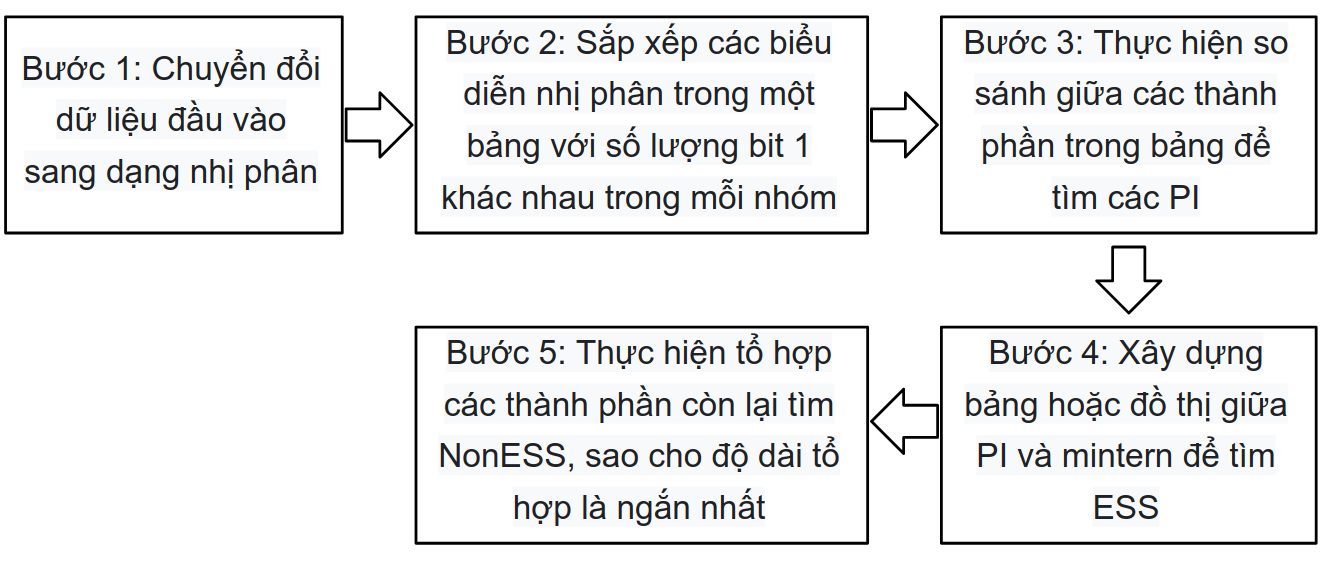
\includegraphics[width=\textwidth]{Image/thuat_toan.png}
	\caption[Sơ đồ trình tự thực hiện giải thuật]{\centering Sơ đồ trình tự thực hiện giải thuật} \label{img:thuat_toan}
\end{figure} \vspace{-0.5cm}
\hspace{0.4cm}Thuật toán Quine-MCluskey \cite{QM:2020} được em thực hiện theo các bước trên hình \ref{img:thuat_toan} với với các dữ liệu đầu vào là: 
\begin{itemize}\vspace{-0.5cm}
 \item Mảng $arr\_input$: là danh sách dữ liệu có thể là dạng mintern $\sum M(1,2,3,4, \dots)$ hay maxtern $\prod M(1,2,3,4, \dots)$.
 \item Biến $type$: để xác định dữ liệu mảng $arr\_input$ trên là dạng mintern hay maxtern hỗ trợ cho việc thực hiện tính toán ($type = 1$: mintern, $type = 2$: maxtern).\\
 Nếu dữ liệu là dạng maxtern thì vẫn thực hiện thuật toán bình thường, chỉ khác ở lúc biểu diễn kết quả.
 \item Mảng $arr\_dont\_care$: là danh sách các don't care.
\end{itemize}
\vspace{0.0cm}
\vspace{-0.5cm}\hspace{0.4cm} Đầu ra là biểu diễn các trường hợp rút gọn hàm logic dưới dạng tổng các tích (SOP) hoặc là tích các tổng (POS).
\newline 
\newline
Từng bước thực hiện:
\begin{itemize} \vspace{-0.5cm}
    \item Bước 1: Ta thực hiện chuyển đổi toàn bộ dữ liệu đầu vào (gồm cả mintern (hoặc maxtern) và don't care) sang dạng số nhị phân.
    \item Bước 2:
    \begin{figure}[H] 
	\centering
	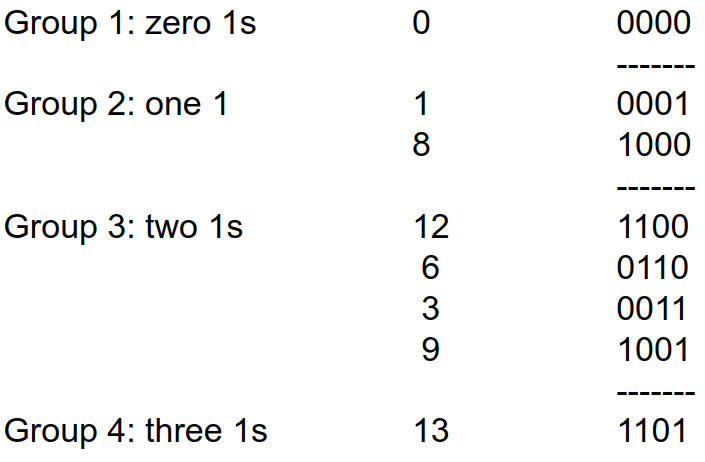
\includegraphics[width=0.6\textwidth]{Image/step_2.png}
	\caption[Minh họa thực hiện phân loại ở bước 2]{\centering Minh họa thực hiện phân loại ở bước 2} \label{img:step_2}
    \end{figure} \vspace{-0.5cm} 
    
    \item Bước 3: 
    \begin{figure}[H] 
	\centering
	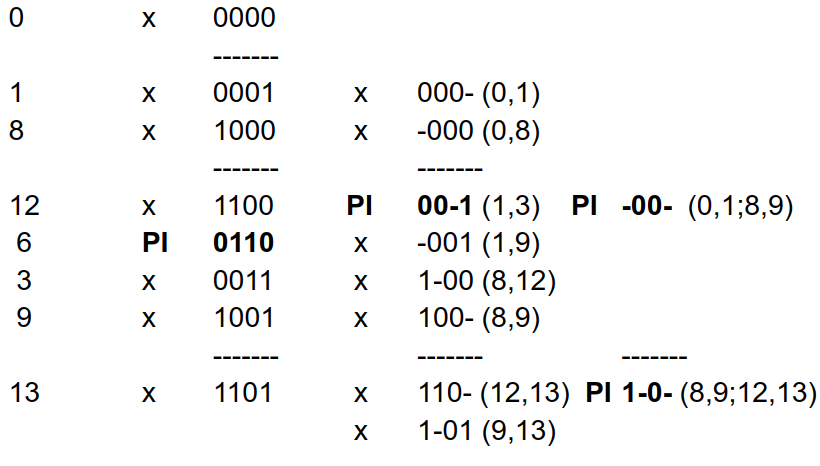
\includegraphics[width=0.6\textwidth]{Image/step_3.png}
	\caption[Minh họa thực hiện bước 3]{\centering Minh họa thực hiện bước 3} \label{img:step_3}
    \end{figure} \vspace{-0.5cm} 
    
    \item Bước 4: 
    \begin{figure}[H] 
	\centering
	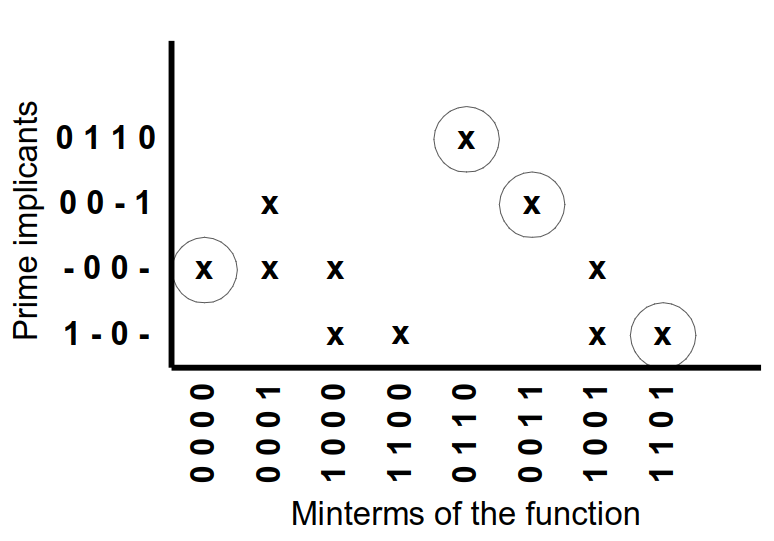
\includegraphics[width=0.6\textwidth]{Image/step_4.png}
	\caption[Minh họa thực hiện bước 4]{\centering Minh họa thực hiện bước 4} \label{img:step_4}
    \end{figure} \vspace{-0.5cm}  
    
    \item Bước 5: Sau bước 4 đã có các ESS, ta tiếp tục thực hiển tổ hợp các PI còn lại sao cho mọi cột mintern trên hình minh họa \ref{img:step_4} được gạch hết và đồng thời số phần tử trong một nhóm tổ hợp là nhỏ nhất (tương tự như phương pháp Petricks \cite{Petrick:2020}). Ta thu được các cặp NonESS kết hợp với ESS tạo thành các hàm logic rút gọn.
    
    
\end{itemize}


\subsection{Kết quả thực hiện}
\begin{enumerate}
    \item \underline{Ví dụ 1}: Thực hiện rút gọn hàm logic: \\   
    $f(A,B,C,D) = \sum m(0,2,4,5,6,9,10) + D(7,11,12,13,14,15)$
    \begin{itemize} 
        \item Thực hiện trên giấy với bìa Karnaugh \cite{KMap:2020} để so sánh kết quả giải thuật:
        \begin{figure}[!h]
        \begin{minipage}[t]{0.5\linewidth}
            \centering
            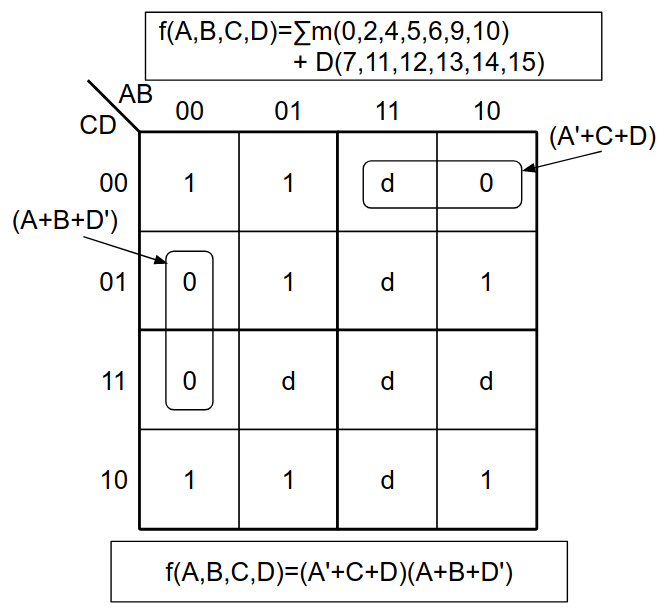
\includegraphics[width=.9\textwidth]{Image/kmap_maxtern_1.png}
            \caption[K-Map dạng POS ví dụ 1]{\centering K-Map dạng POS ví dụ 1}
            \label{img:kmap_maxtern_1}
        \end{minipage}
        \hspace{0.1cm}
        \begin{minipage}[t]{0.5\linewidth} 
            \centering
            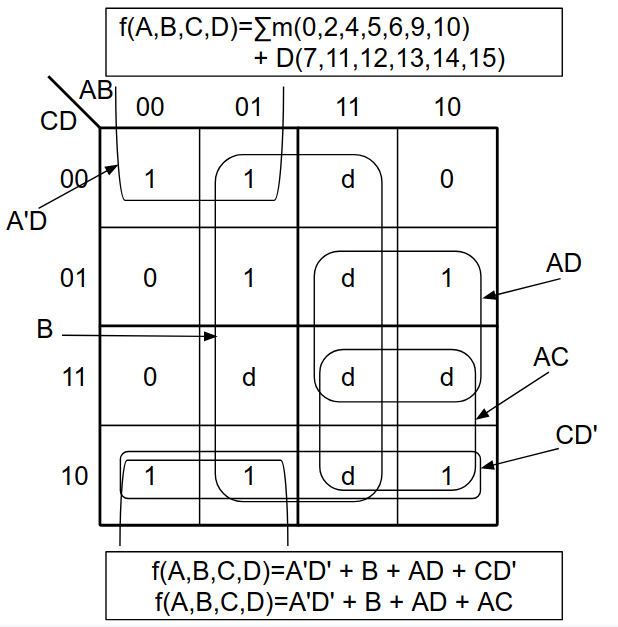
\includegraphics[width=.9\textwidth]{Image/kmap_mintern_1.png}
            \caption[K-Map dạng SOP ví dụ 1]{\centering K-Map dạng SOP ví dụ 1}
            \label{img:kmap_mintern_1}
        \end{minipage}        
        \end{figure}  
        
        \newline 
        \item Nhập dữ liệu đầu vào trên code Python \cite{Python:Ref}: 
        \begin{minted}
        [
        frame=single,
        baselinestretch=1.2,
        fontsize=\footnotesize,
        ] {python}
  arr_mintern = [0,2,4,5,6,9,10]
  arr_dont_care = [7,11,12,13,14,15]
  so_bien = 4
  type = 1 # dữ liệu vào là mintern

  kq = Result(so_bien, arr_mintern, arr_dont_care, type)
  print('Kết quả dạng tổng các tích (SOP): ')
      for result in kq.sop_result():
          print(result)

  print('\nKết quả dạng tích các tổng (POS): ')
      for result in kq.pos_result():
          print(result)
        \end{minted}
        
        \item Kết quả chạy chương trình:
         %Output
        \begin{figure}[H] \vspace{-0.5cm}
    	\centering
    	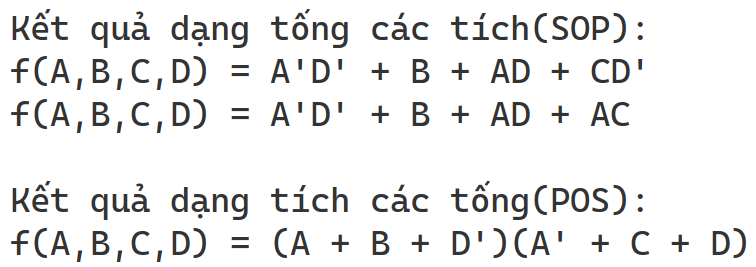
\includegraphics[width=0.7\textwidth]{Image/ket_qua_1.png}
    	\caption[Kết quả thực hiện ví dụ 1]{\centering Kết quả thực hiện ví dụ 1} \label{img:ket_qua_1}
        \end{figure} \vspace{-0.5cm}  
    \end{itemize}
    
    
    % Ví dụ 2:
    \item \underline{Ví dụ 2}: Thực hiện rút gọn hàm logic: \\   
    $f(A,B,C,D) = \prod M(0,1,4,8,10,11,12,14,15)$
    \begin{itemize} 
        \item Thực hiện trên giấy với bìa Karnaugh \cite{KMap:2020} để so sánh kết quả giải thuật:
        \begin{figure}[!h]
        \begin{minipage}[t]{0.5\linewidth}
            \centering
            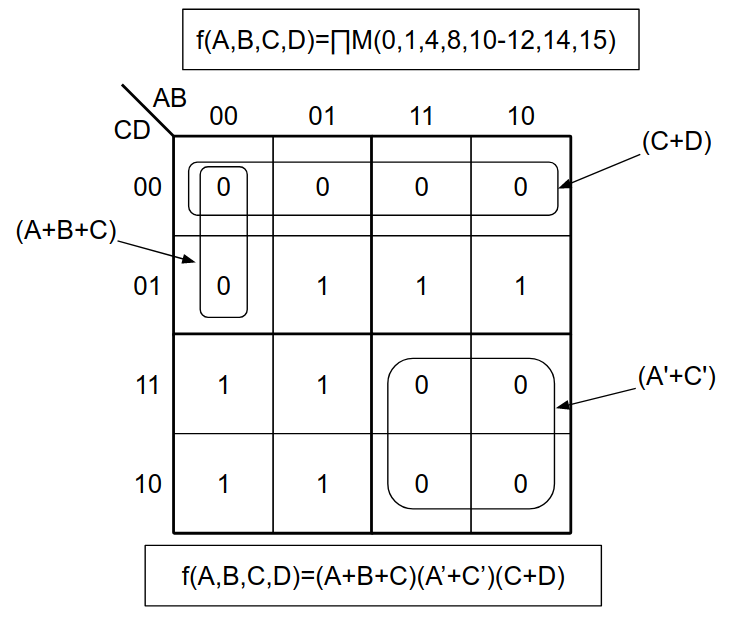
\includegraphics[width=.9\textwidth]{Image/kmap_maxtern_2.png}
            \caption[K-Map dạng POS ví dụ 2]{\centering K-Map dạng POS ví dụ 2}
            \label{img:kmap_maxtern_2}
        \end{minipage}
        \hspace{0.1cm}
        \begin{minipage}[t]{0.5\linewidth} 
            \centering
            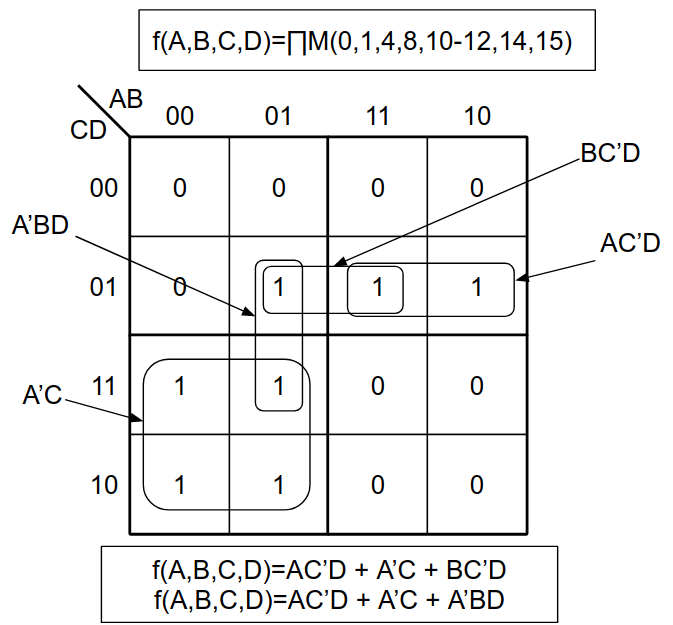
\includegraphics[width=.9\textwidth]{Image/kmap_mintern_2.png}
            \caption[K-Map dạng SOP ví dụ 2]{\centering K-Map dạng SOP ví dụ 2}
            \label{img:kmap_mintern_2}
        \end{minipage}        
        \end{figure}  
        
        \newline
        \item Nhập dữ liệu đầu vào trên code Python \cite{Python:Ref}: 
        \begin{minted}
        [
        frame=single,
        baselinestretch=1.2,
        fontsize=\footnotesize,
        ] {python}
  arr_maxtern = [0,1,4,8,10,11,12,14,15]
  arr_dont_care = []
  so_bien = 4
  type = 2 # dữ liệu vào là maxtern

  kq = Result(so_bien, arr_maxtern, arr_dont_care, type)
  print('Kết quả dạng tổng các tích (SOP): ')
      for result in kq.sop_result():
          print(result)

  print('\nKết quả dạng tích các tổng (POS): ')
      for result in kq.pos_result():
          print(result)
        \end{minted}
        
        \item Kết quả chạy chương trình:
         %Output
        \begin{figure}[H] \vspace{-0.5cm}
    	\centering
    	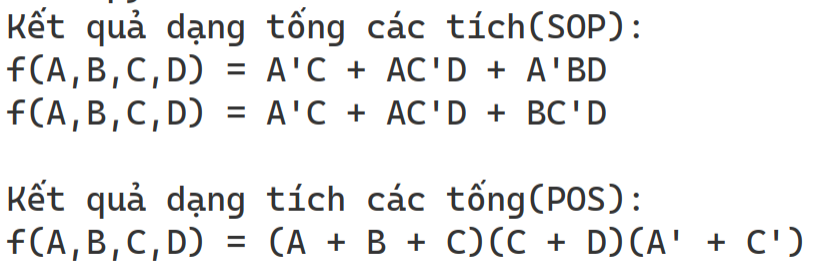
\includegraphics[width=0.7\textwidth]{Image/ket_qua_2.png}
    	\caption[Kết quả thực hiện ví dụ 2]{\centering Kết quả thực hiện ví dụ 2} \label{img:ket_qua_2}
        \end{figure} \vspace{-0.5cm}  
        
    \end{itemize}
    
    
    
    % Ví dụ 3:
    \item \underline{Ví dụ 3}: Thực hiện rút gọn hàm logic 6 biến: \\   
    $f(A,B,C,D) = \sum m(1-9,20-24,27,29,34,36,38,39,42,50) + D(11,15,18,19,45-47,60-63)$
    \begin{itemize} 
        \item Nhập dữ liệu đầu vào trên code Python \cite{Python:Ref}: 
        \begin{minted}
        [
        frame=single,
        baselinestretch=1.2,
        fontsize=\footnotesize,
        ] {python}
  arr_mintern = [1,2,3,4,5,6,7,8,9,20,21,22,23,24,27,29,
            34,36,38,39,42,50]
  arr_dont_care = [11,15,18,19,45,46,47,60,61,62,63]
  so_bien = 6
  type = 1 # dữ liệu vào là mintern

  kq = Result(so_bien, arr_mintern, arr_dont_care, type)

  print('Kết quả dạng tổng các tích (SOP): ')
      for result in kq.sop_result():
          print(result)
        \end{minted}
        
        \item Kết quả chạy chương trình:
         %Output
        \begin{figure}[H] \vspace{-0.5cm}
    	\centering
    	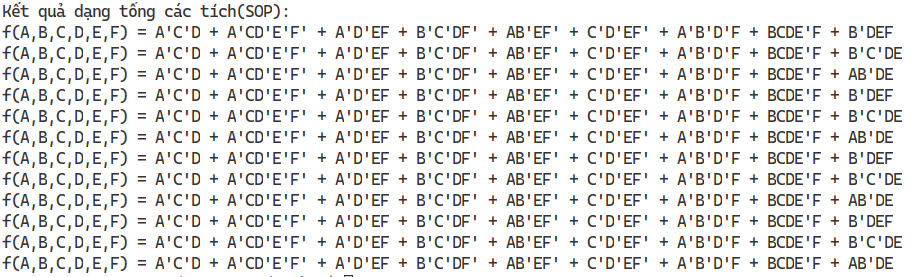
\includegraphics[width=0.85\textwidth]{Image/ket_qua_3.png}
    	\caption[Kết quả thực hiện ví dụ 3]{\centering Kết quả thực hiện ví dụ 3} \label{img:ket_qua_3}
        \end{figure} \vspace{-0.5cm}  
        
    \end{itemize}
\end{enumerate}

\subsection{Nhận xét}
\hspace{0.4cm} 
Em thực hiện thuật toán Quine-MCluskey \cite{QM:2020} trên bằng ngôn ngữ Python \cite{Python:Ref}. \\
Trong bài code, em cài đặt cho phép đầu vào với bất kì số lượng biến, mảng có thể là mintern hoặc maxtern và don't care. Kết quả đầu ra có thế xem được các PI (Prime Implicant), ESS (Essential prime), NonESS (Nonessential prime) và dạng kết quả SOP (tổng các tích) hoặc POS (tích các tổng) thông qua các hàm được cài đặt.


\newpage


% Phụ lục Code 
\section*{\centering PHỤ LỤC}
\addcontentsline{toc}{section}{\numberline{}PHỤ LỤC}
%\listoflistings

\begin{itemize}
    \item Tạo đối tượng \textbf{PhanTu} để lưu chữ các chỉ số, mã nhị phân, biểu diễn dạng maxtern (ví dụ: 1\--\--0 $\rightarrow$ AD', \--001 $\rightarrow$ BCD', \dots), biểu diễn dạng mintern (ví dụ: 1\--\--0 $\rightarrow$ AD', 1\--10 $\rightarrow$ ACD', \dots):
\end{itemize} \vspace{-1.0cm}
% MyClass.py
\begin{minted} 
[frame=single,
baselinestretch=1.2,
fontsize=\footnotesize,
obeytabs=true,
tabsize=20]{python}
# PhanTu là đối tượng để chứa chỉ số mintern, maxtern hoặc don't care  
# Và mã nhị phân tương ứng dạng chuỗi và mã Code (A, B, A', B,...)
class PhanTu: 
    def __init__(self, so_bien, chi_so):
        self.__so_bien = so_bien
        self.__chi_so = [x for x in chi_so]

    # chuyển chỉ số sang mã nhị phân 
    @property
    def code_binary(self):
        if (len(self.__chi_so) > 1): return None 
        str_format = "{0:>0" + str(self.__so_bien) + "s}"
        return str_format.format(bin(int(self.__chi_so[0]))[2:])
        
    # chuyển mã nhị phấn sang kí tự (A, B, A', B',...) dạng mintern
    @property
    def code_mintern(self):
        arr = [chr(ord('A')+i)for i in range(self.__so_bien)]
        arr_code = ''
        binary = self.__ma_nhi_phan
        for i in range(len(binary)):
            if binary[i] != '-':
                if binary[i] == '1': 
                    arr_code += arr[i]
                else: 
                    arr_code += arr[i]+"\'"
        return arr_code

    # chuyển mã nhị phấn sang kí tự (A, B, A', B',...) dạng maxtern 
    @property
    def code_maxtern(self):
        arr = [chr(ord('A')+i)for i in range(self.__so_bien)]
        arr_code = '('
        binary = self.__ma_nhi_phan
        for i in range(len(binary)):
            if binary[i] != '-':
                if binary[i] == '0':
                    arr_code += arr[i]+" + "
                else: 
                    arr_code += arr[i]+"\' + "
        arr_code = arr_code[0:len(arr_code)-3]+")"
        return arr_code 

    @property # Đếm số lượng bit 1 
    def count_bit_one(self):
        return self.__ma_nhi_phan.count('1')

    # Check xem 2 nhóm có khác nhau duy nhất 1 bit hay không
    def check_khac_nhau_1_bit(self, n2):
        ma1 = self.__ma_nhi_phan
        ma2 = n2.__ma_nhi_phan
        count = 0
        for i in range(len(ma1)):
            count += (1 if ma1[i] != ma2[i] else 0)
        return count == 1

    @property # Getter chỉ số
    def p_chi_so(self): return self.__chi_so

    @property # Getter số biến
    def p_so_bien(self): return self.__so_bien

    @property # Getter mã nhị phân
    def p_ma_nhi_phan(self): return self.__ma_nhi_phan
    
    @p_ma_nhi_phan.setter # Setter mã nhị phân
    def p_ma_nhi_phan(self, ma_nhi_phan):
        self.__ma_nhi_phan = ma_nhi_phan 

    # hàm so sánh 2 nhóm (bằng nhau khi có mã nhị phân giống nhau)
    def __eq__(self, other):
        return self.__ma_nhi_phan == other.__ma_nhi_phan
    
    # Hàm hủy bộ nhớ các biến
    def __del__(self):
        del self.__chi_so, self.__ma_nhi_phan, self.__so_bien
\end{minted}

% Các hàm hỗ trợ chương trình
\begin{itemize}
    \item Các hàm chức năng hỗ trợ cho toàn chương trình:
\end{itemize} \vspace{-1.0cm}
\begin{minted}
[
frame=single,
baselinestretch=1.2,
fontsize=\footnotesize,
]
{python}
# Trả về mã nhị phân mới khi 2 nhóm khác nhau duy nhất 1 bit
def ma_nhi_phan_moi(ma1, ma2):
    ma = ''
    for i in range(len(ma1)):
        ma += (ma1[i] if ma1[i]==ma2[i] else '-')
    return ma

# Hàm kiểm tra có tồn tại phần tử trong mảng 
def add_khong_trung(arr, *item):
    if len(arr) == 0:
        for x in item: arr.append(x)
    else:
        for x in item: 
            if arr.count(x) == 0: arr.append(x)

# Hàm kiểm tra có tồn tại phần tử trong mảng hay không
def check_ton_tai(arr, item): 
    if len(arr) == 0: return False 
    return True if arr.count(item) > 0 else False

# Hàm thực hiện tổ hợp các nhóm lại,
# Loại bỏ nhóm trùng và lấy danh sách các nhóm có độ dài ngắn nhất 
def to_hop_nhom(arr_temp):
    min_length = len(arr_temp)
    arr_tron = []
    arr_so_luong_moi_hang = []
    arr_choice = [0]*len(arr_temp)
    so_lan_lap = 1
    for i in range(len(arr_temp)):
        so_lan_lap *= len(arr_temp[i])
        arr_so_luong_moi_hang.append(len(arr_temp[i]))
    
    index = 0
    while index < so_lan_lap:
        arr_row = []
        for i in range(len(arr_temp)):
            add_khong_trung(arr_row, arr_temp[i][arr_choice[i]])
        index += 1 
        check_nho = True 
        for i in range(len(arr_temp)-1, -1, -1):
            arr_choice[i] += 1
            if arr_choice[i] == arr_so_luong_moi_hang[i]:
                arr_choice[i] = 0
            else: 
                check_nho = False
        if len(arr_row) < min_length:
            min_length = len(arr_row)
        arr_tron.append(arr_row)
    return [x for x in arr_tron if min_length == len(x)]
\end{minted}

% Class xử lý 
\begin{itemize}
    \item Class \textbf{XuLy} chức năng xử lý dữ liệu đầu vào để đưa ra các PI (Prime Implicant), ESS (Essential Prime) và NonESS (Nonessential Prime):
\end{itemize} \vspace{-1.0cm}
\begin{minted}
[
frame=single,
baselinestretch=1.2,
fontsize=\footnotesize,
]
{python}
class XuLy:
    # arr truyền vào là mintern
    def __init__(self, so_bien, arr, arr_dont_care):
        arr_join = sorted(arr+arr_dont_care)
        self.mintern = arr 
        self.so_bien = so_bien
        arr = []
        for item in arr_join: 
            item = [item]
            n = PhanTu(so_bien, item)
            n.p_ma_nhi_phan = n.code_binary
            arr.append(n)
        self.arr_nhom = arr
    
    # Hàm trả về mảng mà số lượng bít 1 chung 1 nhóm 
    # Và được SX theo số lượng bit 1 tăng dần 
    def arr_theo_sl_bit_1(self):
        arr = []
        for i in range(self.so_bien+1):
            arr_tmp=[x for x in self.arr_nhom if x.count_bit_one==i]
            arr.append(arr_tmp)
        # chuyển mảng 2 chiều về 1 chiều
        return list(it.chain.from_iterable(arr))  

    # Hàm trả về các Prime Implicant (PI)
    def arr_prime_implicant(self):
        arr_all = self.arr_nhom.copy()
        arr_pi = [] # Chứa các phần tử không có cặp 
        arr_co_cap = []
        arr_new = []
        while True: 
            check = False
            size = len(arr_all)
            for i in range(size-1):
                dem = 0
                nhom_A = arr_all[i]
                for j in range(i+1, size):
                    nhom_B = arr_all[j]
                    if nhom_A.check_khac_nhau_1_bit(nhom_B):
                        # Thêm 2 nhóm này vào mảng có cặp
                        add_khong_trung(arr_co_cap, nhom_A, nhom_B)
                        check = True
                        dem += 1
                        
                        chi_so = nhom_A.p_chi_so + nhom_B.p_chi_so
                        ma_nhom_a = nhom_A.p_ma_nhi_phan 
                        ma_nhom_b = nhom_B.p_ma_nhi_phan
                        maNP = ma_nhi_phan_moi(ma_nhom_a, ma_nhom_b)

                        nhom_new = PhanTu(self.so_bien, chi_so)
                        nhom_new.p_ma_nhi_phan = maNP
                        add_khong_trung(arr_new, nhom_new)

                if dem==0 and(not check_ton_tai(arr_co_cap, nhom_A)):
                    add_khong_trung(arr_pi, nhom_A)
            if not check_ton_tai(arr_co_cap, arr_all[size - 1]):
                add_khong_trung(arr_pi, arr_all[size - 1])
            if not check: 
                for x in arr_all: add_khong_trung(arr_pi, x)
                break
            arr_all = arr_new.copy()
            arr_new = []
            arr_co_cap = [] 
        return arr_pi

    # Hàm trả về các Essential 
    def arr_essential(self):
        arr_pi = self.arr_prime_implicant()
        arr_mintern = self.mintern.copy()
        arr_mintern.sort()

        size = len(arr_mintern)
        arr_chi_so = [x.p_chi_so for x in arr_pi]

        # arr_count là mảng đối chiếu với mintern 
        arr_count = [0]*size 
        for i in range(size):
            for arr_num in arr_chi_so:
                for j in range(len(arr_num)):
                    if arr_num[j] == arr_mintern[i]: 
                        arr_count[i] += 1 
                    else: 
                        arr_count[i] += 0
        
        arr_ess = []
        for i in range(size):
            count = arr_count[i] 
            value = arr_mintern[i]
            if count == 1:
                for item in arr_pi:
                    if item.p_chi_so.count(value) > 0: 
                        add_khong_trung(arr_ess, item)
        return arr_ess

    
    # Hàm trả về các cặp nonEssential (tổ hợp nhỏ nhất)
    def arr_non_essential(self):
        cot_con_trong = self.mintern.copy()
        arr_ess = self.arr_essential()
        arr_pi = self.arr_prime_implicant() 

        for item in arr_ess:
            for num in item.p_chi_so:
                if cot_con_trong.count(num) > 0:
                    cot_con_trong.remove(num)
        # Nếu không còn cột nào trống thì trả về mảng rỗng
        if len(cot_con_trong) == 0: return []
        
        # Lấy mảng để tổ hợp 
        arr_temp = []
        con_lai = [x for x in arr_pi if x not in arr_ess]
        for num in cot_con_trong:
            arr_row = []
            for item in con_lai:
                if item.p_chi_so.count(num) > 0:
                    add_khong_trung(arr_row, item)
            arr_temp.append(arr_row)
        return to_hop_nhom(arr_temp)
\end{minted}

% Class Result.py
\begin{itemize}
    \item Class \textbf{Result} chức năng in và xử lý kết quả đầu ra:
\end{itemize} \vspace{-1.0cm}
\begin{minted}
[
frame=single,
baselinestretch=1.2,
fontsize=\footnotesize,
]
{python}
class Result:
    # Với arr_input là các mảng truyền vào dạng các mintern or maxtern
    # type: loại input truyền vào 
    # type = 1 thì input là mintern
    # type = 2 thì input là maxtern
    def __init__(self,so_bien, arr_input, arr_dont_care, type):
        self.arr_dont_care = arr_dont_care.copy()
        self.so_bien = so_bien
        self.type = type
        if type == 1:
            self.arr_maxtern = [x for x in range(2**so_bien)
            if x not in arr_input and x not in arr_dont_care]
            self.arr_mintern = arr_input.copy()
        elif type == 2:
            self.arr_mintern = [x for x in range(2**so_bien) 
            if x not in arr_input and x not in arr_dont_care]
            self.arr_maxtern = arr_input.copy()
        
    # Lấy f(A,B,C,D,....) = 
    def __function(self):
        arr = [chr(ord('A')+i) for i in range(self.so_bien)]
        fStr = "f(" 
        for i in range(len(arr) - 1):
            fStr += arr[i] + ","
        return fStr + arr[len(arr) - 1] + ") = "

    # Hàm trả về mảng các kết quả dạng SOP (tổng các tích) mintern
    def sop_result(self):
        xl = XuLy(self.so_bien, self.arr_mintern, self.arr_dont_care)
        arr_ess = xl.arr_essential()
        arr_non_ess = xl.arr_non_essential()

        str_temp = self.__function()
        for item in arr_ess:
            str_temp += item.code_mintern + " + "
        if len(arr_non_ess) == 0: return [str_temp[:len(str_temp)-3]]
        
        arr_result = []
        for item in arr_non_ess:
            str_  = str_temp 
            for x in item: str_ += x.code_mintern + " + "
            arr_result.append(str_[:len(str_)-3])
        return arr_result

    # Hàm trả về mảng các kết quả dạng POS (tích các tổng) maxtern
    def pos_result(self):
        xl = XuLy(self.so_bien, self.arr_maxtern, self.arr_dont_care)
        arr_ess = xl.arr_essential()
        arr_non_ess = xl.arr_non_essential()

        str_temp = self.__function()
        for item in arr_ess:
            str_temp += item.code_maxtern
        if len(arr_non_ess) == 0: return [str_temp]
        
        arr_result = []
        for item in arr_non_ess:
            str_  = str_temp 
            for x in item: str_ += x.code_maxtern
            arr_result.append(str_)
        return arr_result
\end{minted}

% Class main.py
\begin{itemize}
    \item Phần code để test chương trình và xem kết quả thực hiện:
\end{itemize} \vspace{-1.0cm}
\begin{minted}
[
frame=single,
baselinestretch=1.2,
fontsize=\footnotesize,
]
{python}
arr_input = [2, 4, 5, 6, 10, 0, 9]
arr_dont_care = [7, 11, 12, 13, 14, 15]
so_bien = 4

# type = 1: arr_input là mintern 
# type = 2: arr_input là maxtern 
kq = Result(so_bien, arr_input, arr_dont_care, type=1)
print('Kết quả dạng tổng các tích: ')
for i in kq.sop_result():
    print(i)

print('Kết quả dạng tích các tổng: ')
for i in kq.pos_result():
    print(i)
\end{minted}

\newpage

% Reference
\addcontentsline{toc}{section}{\numberline{}TÀI LIỆU THAM KHẢO}
\bibliographystyle{IEEEtran}
\bibliography{tailieuthamkhao}

\end{document}